%!TEX root = ../thesis.tex
\section{ニューラルネットワーク}
ニューラルネットワークは，脳の神経回路網を模した数理モデルであり，多層構造を持つことで複雑な非線形関数を近似する能力を有する．入力層から出力層へ信号を伝播させ，誤差逆伝播法により結合重みを調整することで学習を行う．本研究では，強化学習における方策や価値関数の近似器として深層ニューラルネットワークを用い，高次元なセンサ情報から適切な制御入力を生成する非線形写像を構築する．

\begin{figure}[H]
  \centering
 \includegraphics[keepaspectratio, scale=0.8]
      {images/RaspberryPiMouse.png}
 \caption{Example}
 \label{Fig:Example}
\end{figure}

\section{強化学習}
強化学習は，エージェントが環境と相互作用しながら，試行錯誤を通じて累積報酬を最大化する行動方針を学習する枠組みである．マルコフ決定過程として定式化され，状態，行動，報酬により問題が定義される．教師データを与えられるのではなく，自らの行動結果として得られる報酬をフィードバックとして学習を進めるため，未知の環境や複雑なタスクに対しても適応的な制御則を獲得することが可能である．
\begin{figure}[H]
  \centering
 \includegraphics[keepaspectratio, scale=0.8]
      {images/RaspberryPiMouse.png}
 \caption{Example}
 \label{Fig:Example}
\end{figure}

\section{NVIDIA Isaac Lab}
NVIDIA Isaac Lab\cite{mittal2025isaaclab}は，Omniverse上に構築されたロボット学習用シミュレーションフレームワークである．PhysXによる高精度な物理演算とGPUによる並列処理を組み合わせることで，数千体のロボットを同時にシミュレーション可能とする．これにより，深層強化学習に不可欠な膨大な試行回数を短時間で確保でき，現実世界では困難な大規模なデータ収集と効率的な学習を実現する．
\begin{figure}[H]
  \centering
 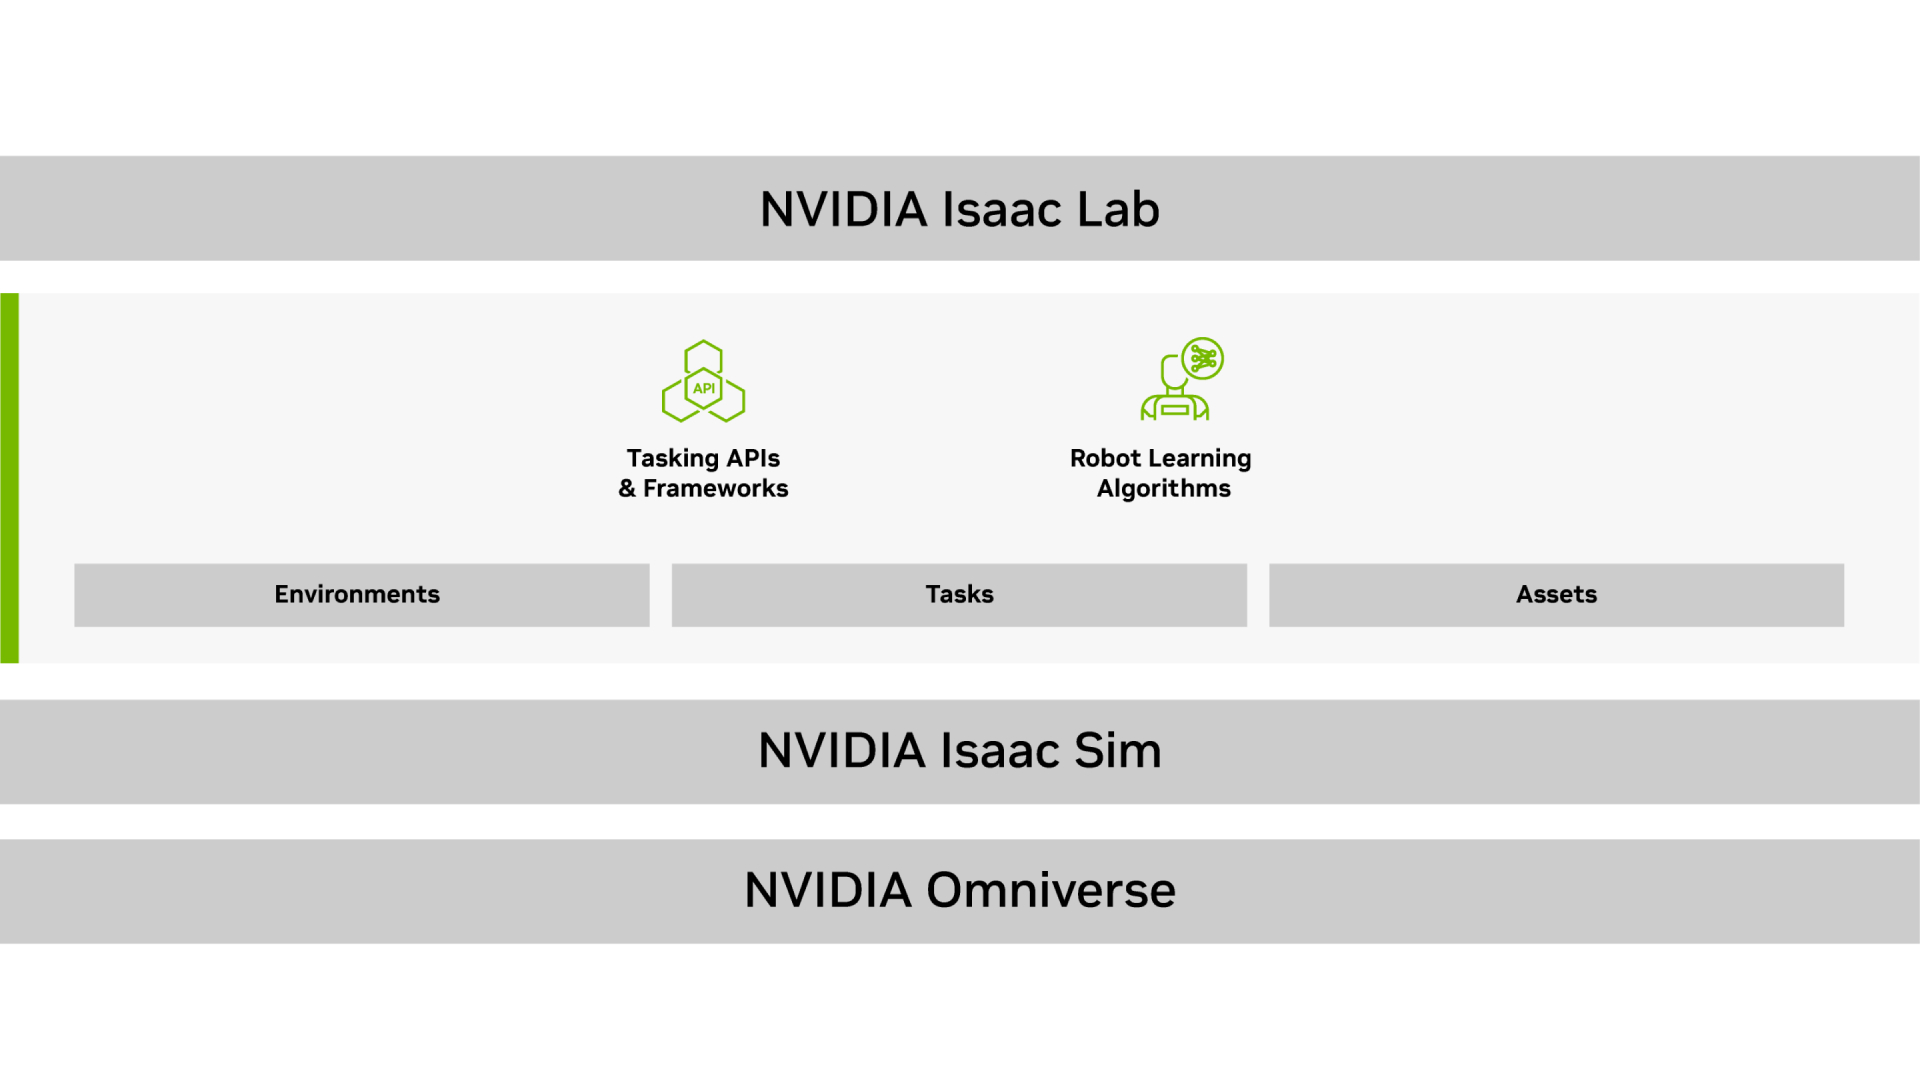
\includegraphics[keepaspectratio, scale=0.2]
      {images/png/how-nvidia-isaac-lab-works.png}
 \caption{How NVIDIA Isaac Lab Works}
 \label{Fig:nvidia-isaac-lab}
\end{figure}
\section{深層強化学習による歩行制御}
深層強化学習を用いた歩行制御は，試行錯誤を通じてロバストな運動機能を獲得する手法である．Rudinら\cite{rudin2021learning}は，GPUによる大規模並列シミュレーションを活用し，数千体のロボットを同時に学習させることで，不整地踏破可能な制御則を数分で獲得できることを示した．
\begin{figure}[H]
  \centering
 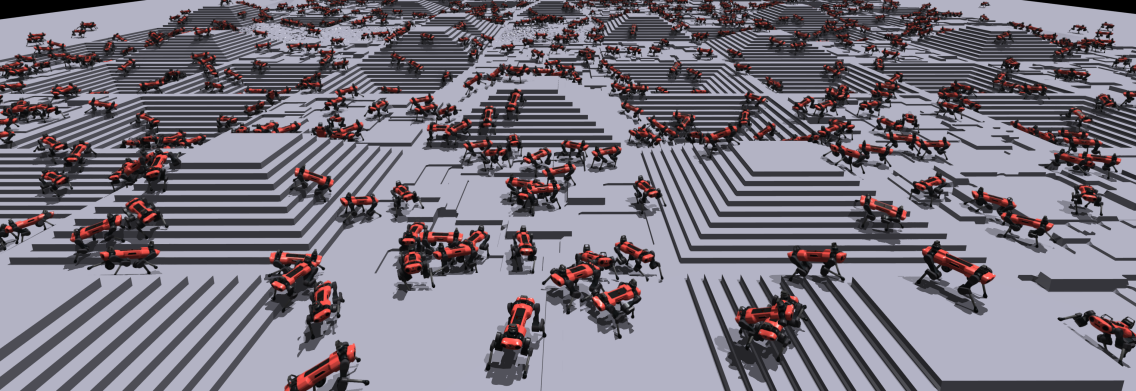
\includegraphics[keepaspectratio, scale=0.8]
      {images/png/anymal.png}
 \caption{Learning to Walk in Minutes Using Massively Parallel Deep Reinforcement Learning (source: \cite{rudin2021learning})}
 \label{Fig:anymal}
\end{figure}

\section{報酬関数の設計}
報酬関数は，強化学習においてエージェントの行動を評価し，学習の方向性を決定づける極めて重要な要素である．歩行制御では，目標速度への追従，転倒回避，エネルギー効率，動作の自然さなど，競合し得る複数の要求を報酬項として適切に設計・重み付けする必要がある．適切な報酬設計なしには意図した動作の獲得は困難であり，各報酬項が学習結果に与える影響やトレードオフを理解することは不可欠である．


\newpage
